\documentclass{standalone} 
\usepackage{tikz}
\usetikzlibrary{spath3,intersections}
\usetikzlibrary{decorations.pathreplacing,decorations.markings}
\tikzset{
  % style to apply some styles to each segment of a path
  on each segment/.style={
    decorate,
    decoration={
      show path construction,
      moveto code={},
      lineto code={
        \path [#1]
        (\tikzinputsegmentfirst) -- (\tikzinputsegmentlast);
      },
      curveto code={
        \path [#1] (\tikzinputsegmentfirst)
        .. controls
        (\tikzinputsegmentsupporta) and (\tikzinputsegmentsupportb)
        ..
        (\tikzinputsegmentlast);
      },
      closepath code={
        \path [#1]
        (\tikzinputsegmentfirst) -- (\tikzinputsegmentlast);
      },
    },
  },
  % style to add an arrow in the middle of a path
  mid arrow/.style={postaction={decorate,decoration={
        markings,
        mark=at position .55 with {\arrow[#1]{stealth}}
      }}},
}
\tikzset{
    bridge/.style 2 args={
        spath/split at intersections with={#1}{#2},
        spath/insert gaps after components={#1}{5pt},
        spath/join components upright with={#1}{myarc},
        spath/split at intersections with={#2}{#1},
        spath/insert gaps after components={#2}{4pt},
    }
}
\begin{document}
    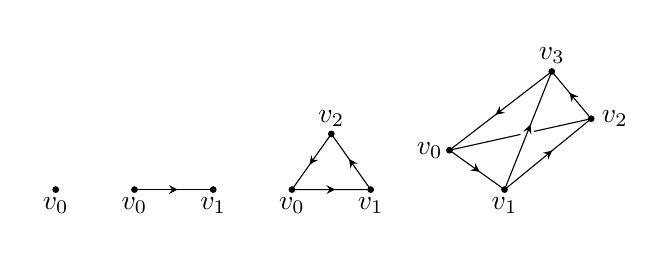
\begin{tikzpicture}
        %Primer simplejo
        \fill[draw] (-1,0) circle (1pt); 
        \node[circle] (v_0) at (-1,-0.2){$v_0$} coordinate (v_0_0);

        %Segundo simplejo
        \fill[draw] (0,0) circle (1pt); 
        \node[circle] (v_0) at (0,-0.2){$v_0$} coordinate (v_0_1);

        \fill[draw] (1,0) circle (1pt); 
        \node[circle] (v_1) at (1,-0.2){$v_1$} coordinate (v_1_1);

        \draw[postaction={on each segment={mid arrow=black}}] (0,0) -- (1,0);

        %Tercer simplejo

        \fill[draw] (2,0) circle (1pt); 
        \node[circle] (v_0) at (2,-0.2){$v_0$} coordinate (v_0_2);

        \fill[draw] (3,0) circle (1pt); 
        \node[circle] (v_1) at (3,-0.2){$v_1$} coordinate (v_1_2);

        \fill[draw] (2.5,0.707) circle (1pt); 
        \node[circle] (v_1) at (2.5,0.907){$v_2$} coordinate (v_2_2);

        \draw[postaction={on each segment={mid arrow=black}}] (2,0) -- (3,0) --  (2.5,0.707) -- (2,0);

        %Cuarto Simplejo

        \fill[draw] (4,0.5) circle (1pt); 
        \node[circle] (v_0) at (3.75,0.5){$v_0$};

        \fill[draw] (4.7,0) circle (1pt); 
        \node[circle] (v_1) at (4.7,-0.2){$v_1$};

        \fill[draw] (5.8,0.9) circle (1pt); 
        \node[circle] (v_2) at (6.1,0.9){$v_2$};

        \fill[draw] (5.3,1.5) circle (1pt); 
        \node[circle] (v_3) at (5.3,1.7){$v_3$};

        \draw[postaction={on each segment={mid arrow=black}}] (4,0.5) -- (4.7,0) --  (5.8,0.9) -- (5.3,1.5) -- (4,0.5);

        \path[spath/save=over] (4,0.5) --  (5.8,0.9);

        \path[spath/save=under] (4.7,0) --  (5.3,1.5);

        \tikzset{bridge={over}{under}}
        \draw[spath/use=over];
        \draw[spath/use=under];

        \path[postaction={on each segment={mid arrow=black}}] (4.7,0) --  (5.3,1.5);

    \end{tikzpicture}
\end{document}